The purpose of this lecture is to introduce some area problem solving techniques that extend beyond the basic formulas for fundamental shapes.
	
	\subsection{Traditional Equations}
	\textbf{Heron's Formula} \textit{The area of a triangle whose sides have lengths $a$, $b$, and $c$ is
  $$ A = \sqrt{s(s-a)(s-b)(s-c)}$$}	
	
	\begin{problem}
	Find the area of a triangle with side lengths 5, 7, 8.
	\end{problem}
	
	\begin{problem}
	Find the area of a triangle with side lengths 13, 14, 15.
	\end{problem}
	
	\noindent \textbf{Brahmagupta's Theorem} \textit{The area $K$ of a cyclic quadrilateral whose sides have lengths $a$, $b$, $c$, $d$ as
  $$ K=\sqrt{(s-a)(s-b)(s-c)(s-d)}$$}

	\begin{problem}
	Find the area of quadrilateral $ABCD$ if it is inscribed in the circle below.
	\begin{center}
	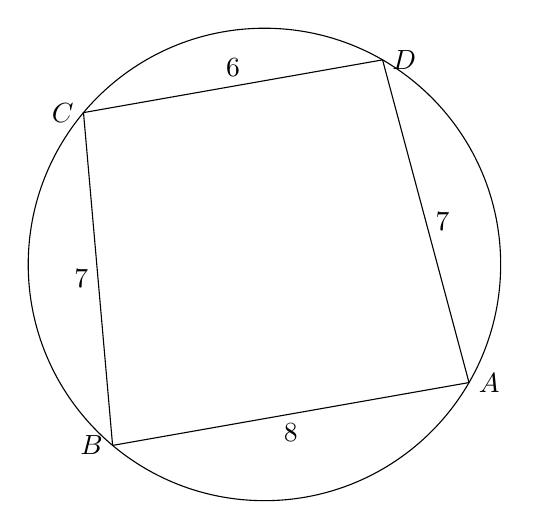
\begin{tikzpicture}
		\draw (0,0) circle  [radius = 3cm];
		\draw (230:3cm) node[left] {$B$};
		\draw (140:3cm) node[left] {$C$};
		\draw (60:3cm) node[above, right] {$D$};
		\draw (-30:3cm) coordinate (a) node[right] {$A$}  --
		 (230:3cm) coordinate (b) node[midway, below] {$8$}  --
		(140:3cm) coordinate (c) node[midway, left] {$7$} --
		(60:3cm) coordinate (d) node[midway, above] {$6$}-- (-30:3cm) coordinate (e) node[midway, right] {$7$};
	\end{tikzpicture}
	\end{center}
	\end{problem}
	
	\clearpage

	\subsection{Pick's Theorem}
	\begin{theorem}
	Given a simple polygon constructed on a unit grid such that all the polygon's vertices are lattice points, the area of this polygon is 
    $$A = i + \frac{b}{2} - 1, $$
		where $i$ is the number of lattice points in the interior located in the polygon and the $b$ is the number of lattice points on the boundary of the polygon.
	\end{theorem}
	%know how to do the proof
	
	\begin{problem}
	What is the area of the polygon in the diagram below? (this is a unit square grid)
	\begin{center}
	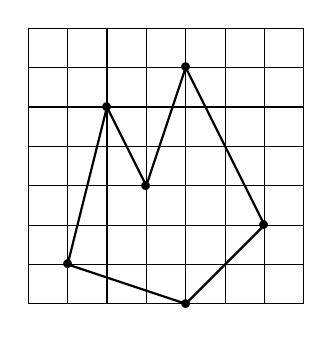
\begin{tikzpicture}[scale=0.5]
			\draw (0,0) grid (7,7);
			\draw (1,1) node[scale=3]{.};
			\draw [thick] (1,1)--(2,5);
			\draw (2, 5) node[scale=3]{.};
			\draw [thick] (2, 5)--(3, 3);
			\draw (3,3) node[scale=3]{.};
			\draw [thick] (3,3)--(4, 6);
			\draw (4, 6) node[scale=3]{.};
			\draw [thick] (4, 6)--(6, 2);
			\draw (6, 2) node[scale=3]{.};
			\draw [thick] (6,2)--(4,0);
			\draw (4,0) node[scale=3]{.};
			\draw [thick] (4,0)--(1,1);
	\end{tikzpicture}
	\end{center}
	\end{problem}
	
	\begin{problem}
	What is the area of the polygon in the diagram below? (this is a unit square grid)
	\begin{center}
	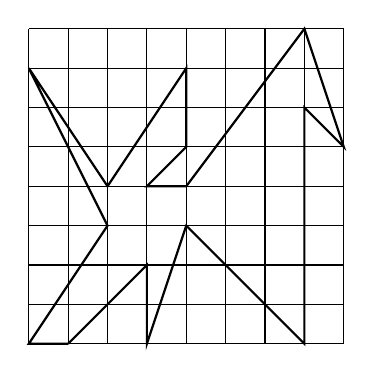
\begin{tikzpicture}[scale=0.5]
		\draw (0,0) grid (8,8);
		\draw [thick] (1,0)--(3,2)--(3,0)--(4,3)--(7,0)--(7,6)--(8,5)--(7,8)--(4,4)--(3,4)--(4,5)--(4,7)--(2,4)--(0,7)--(2,3)--(0,0)--(1,0);
	\end{tikzpicture}
	\end{center}
	\end{problem}

	\subsection{Shoelace Theorem}
	\begin{theorem}
	Suppose the polygon $P$ has vertices $(a_1, b_1)$, $(a_2, b_2)$, ... , $(a_n, b_n)$, listed in clockwise order. Then the area of $P$ is
	\[\dfrac{1}{2} |(a_1b_2 + a_2b_3 + \cdots + a_nb_1) - (b_1a_2 + b_2a_3 + \cdots + b_na_1)|\] 
	\end{theorem}
	
	In case you're wondering where the shoelace formula gets its name, it's because when you list out the coordinates in a matrix,
	 $$\begin{bmatrix} a_1 & b_1 \\ a_2 & b_2\\ \vdots & \vdots \\ a_n & b_n \end{bmatrix},$$
	you'll find out that the multiplication is in a shoelace cross pattern.
	
	\clearpage
	\begin{problem}
	Find the area of the following polygon.
	\begin{center}
	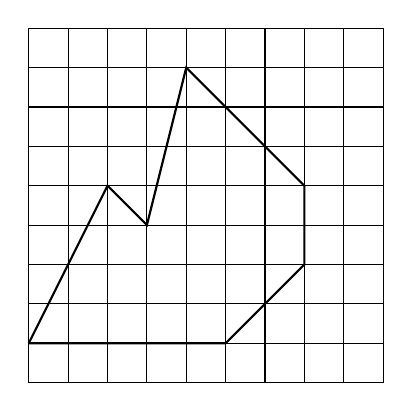
\begin{tikzpicture}[scale=0.5]
	\draw (0,0) grid (9,9);
	\draw [thick] (0,1)--(2, 5)--(3,4)--(4,8)--(6,6)--(7,5)--(7,3)--(6,2)--(5,1)--(3,1)--(0,1);
	\end{tikzpicture}
	\end{center}
	\end{problem}
	
	\begin{problem}
	Find the area of the following polygon with the given coordinates: $(1.2,1), (2.4, 0.5), (8,3.2), \\ (7,6.5), (6,7.2), (3,7.6), (1.2,1) $
	\begin{center}
	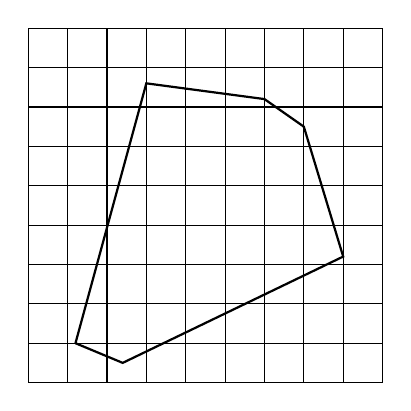
\begin{tikzpicture}[scale=0.5]
	\draw (0,0) grid (9,9);
	\draw [thick] (1.2,1)--(2.4, 0.5)--(8,3.2)--(7,6.5)--(6,7.2)--(3,7.6)--(1.2,1);
	
	\end{tikzpicture}
	\end{center}
	\end{problem}
	
	\subsection{Problems}
	\begin{problem}
	An equiangular octagon has four sides of length 1 and four sides of length $\frac{\sqrt{2}}{2}$, arranged so that no two consecutive sides have the same length. What is the area of the octagon?

$\mathrm{(A) \ } \frac72\qquad \mathrm{(B) \ } \frac{7\sqrt2}{2}\qquad \mathrm{(C) \ } \frac{5+4\sqrt2}{2}\qquad \mathrm{(D) \ } \frac{4+5\sqrt2}{2}\qquad \mathrm{(E) \ } 7$ 
	\end{problem}
	
	\begin{problem}
	Points $E$ and $F$ are located on square $ABCD$ so that $\triangle BEF$ is equilateral. What is the ratio of the area of $\triangle DEF$ to that of $\triangle ABE$? 
	
	\begin{center}
	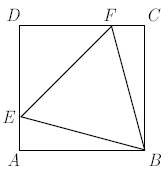
\includegraphics[width=1.6in]{squareTri}
	\end{center}
	\end{problem}
	
	\begin{problem}
	A circle is inscribed in a square, then a square is inscribed in this circle, and finally, a circle is inscribed in this square. What is the ratio of the area of the smaller circle to the area of the larger square?

$\mathrm{(A)} \frac{\pi}{16} \qquad \mathrm{(B)} \frac{\pi}{8} \qquad \mathrm{(C)} \frac{3\pi}{16} \qquad \mathrm{(D)} \frac{\pi}{4} \qquad \mathrm{(E)} \frac{\pi}{2}$
	\end{problem}
	
	\clearpage
	\begin{problem}
	Given that the area of $\triangle ABC$ is 196, and $DB = 6AD$, find the area of $\triangle CDB$.
	\begin{center}
	\begin{tikzpicture}
		\draw (0,0) node [below] {$A$};
		\draw (7,0) node [below]{$B$};
		\draw (5,3) node [above]{$C$}; 
		\draw (1,0) node [below]{$D$};
		\draw (0,0)--(7,0)--(5,3)--(0,0);
		\draw (5,3)--(1,0);
	\end{tikzpicture}
	\end{center}
	\end{problem}
	
	\vspace{0.5in}
	
	\begin{problem}
	Given that $AB=$ and $BC=$, find the area of the shaded region.
	\begin{center}
		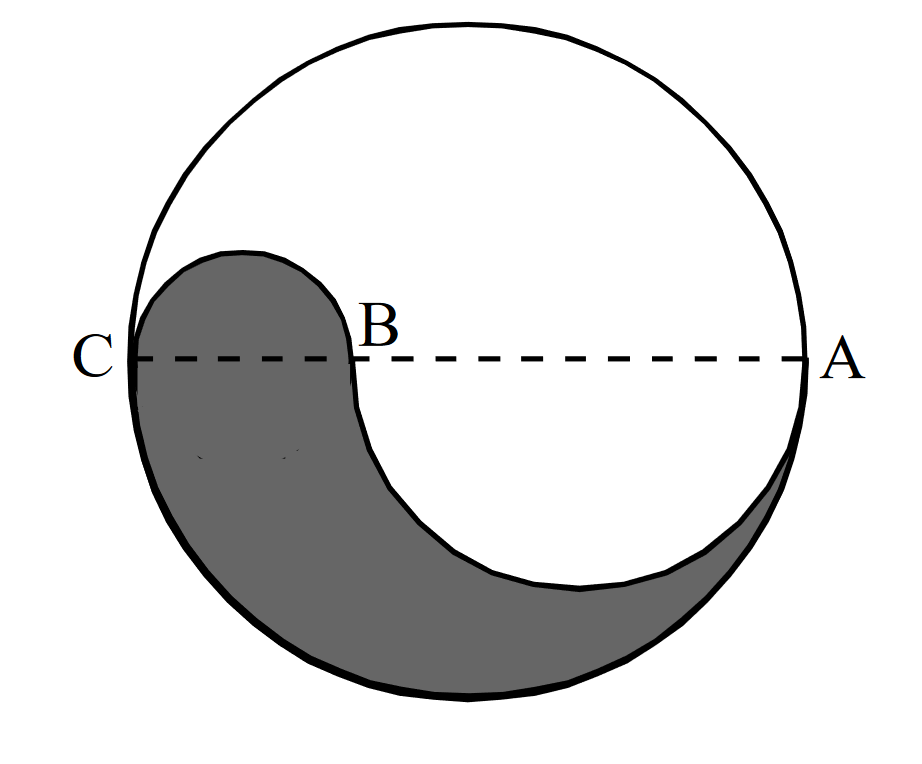
\includegraphics[width=2in]{circle11}
	\end{center}
	\end{problem}
	
	\vspace{0.6in}
	
	\begin{problem}
	Find the area of the shaded region.
	\begin{center}
		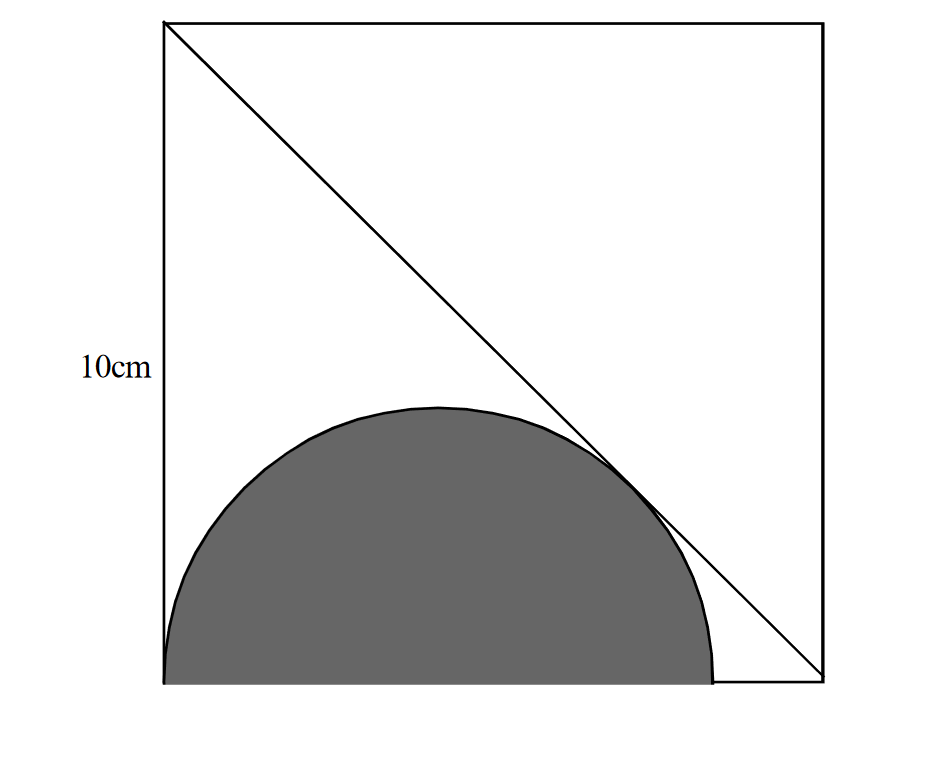
\includegraphics[width=3in]{circle2}
	\end{center}
	\end{problem}
	
	\clearpage
	\begin{problem}
	Find the area of the shaded region.
	\begin{center}
		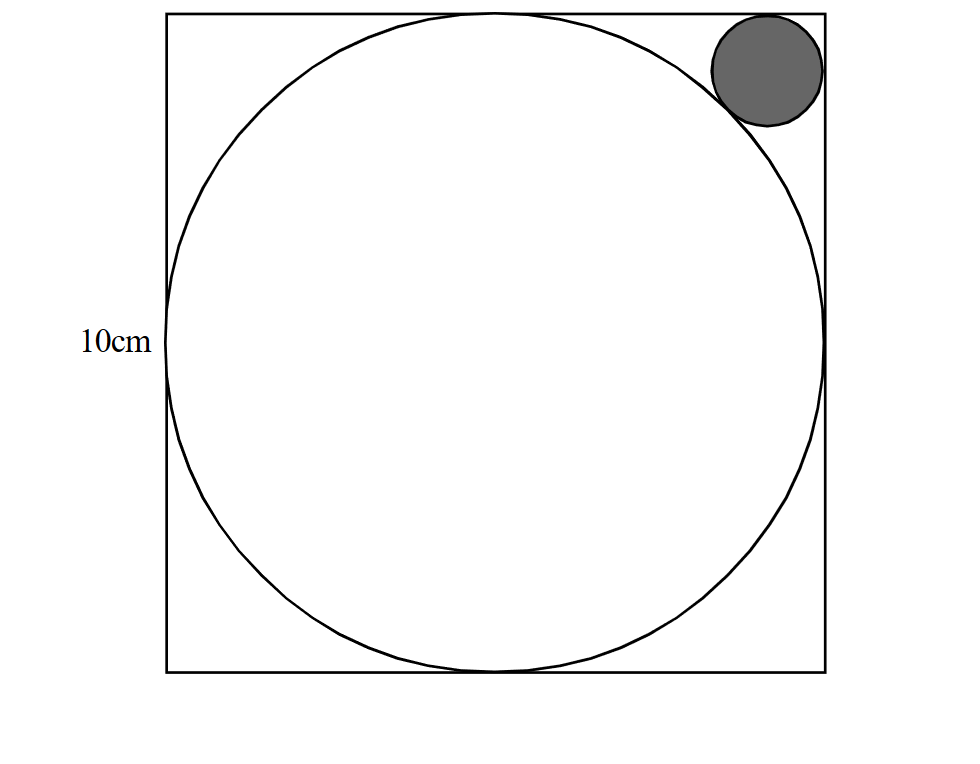
\includegraphics[width=3in]{circle3}
	\end{center}
	\end{problem}
	
	\vspace{1.5in}
	
	\begin{problem}
	Find the area of the shaded region.
	\begin{center}
		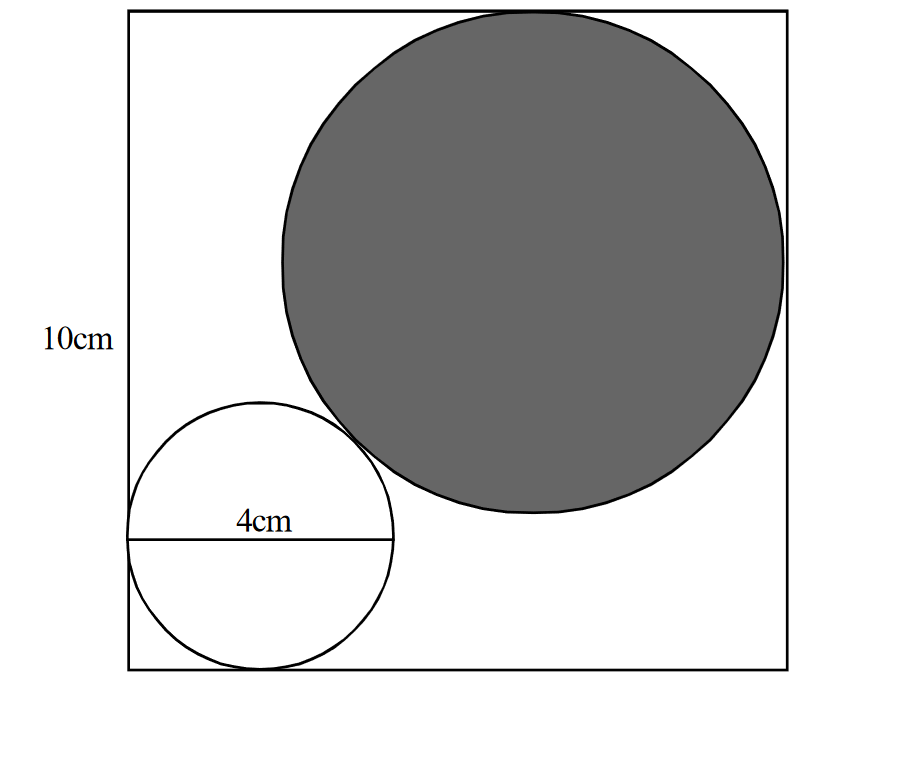
\includegraphics[width=3in]{circle4}
	\end{center}
	\end{problem}
	
	\clearpage
	\begin{problem}
	Find the area of the shaded region.
	\begin{center}
		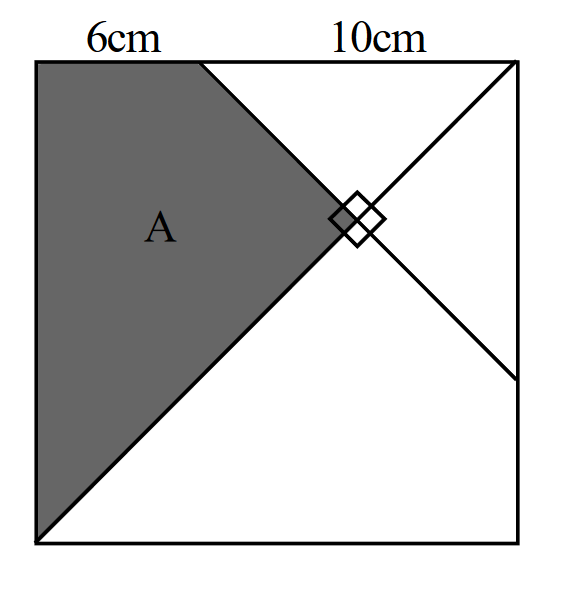
\includegraphics[width=3in]{square}
	\end{center}
	\end{problem}
	
	\vspace{1in}
	
	\begin{problem}
	Find the area of the shaded region.
	\begin{center}
		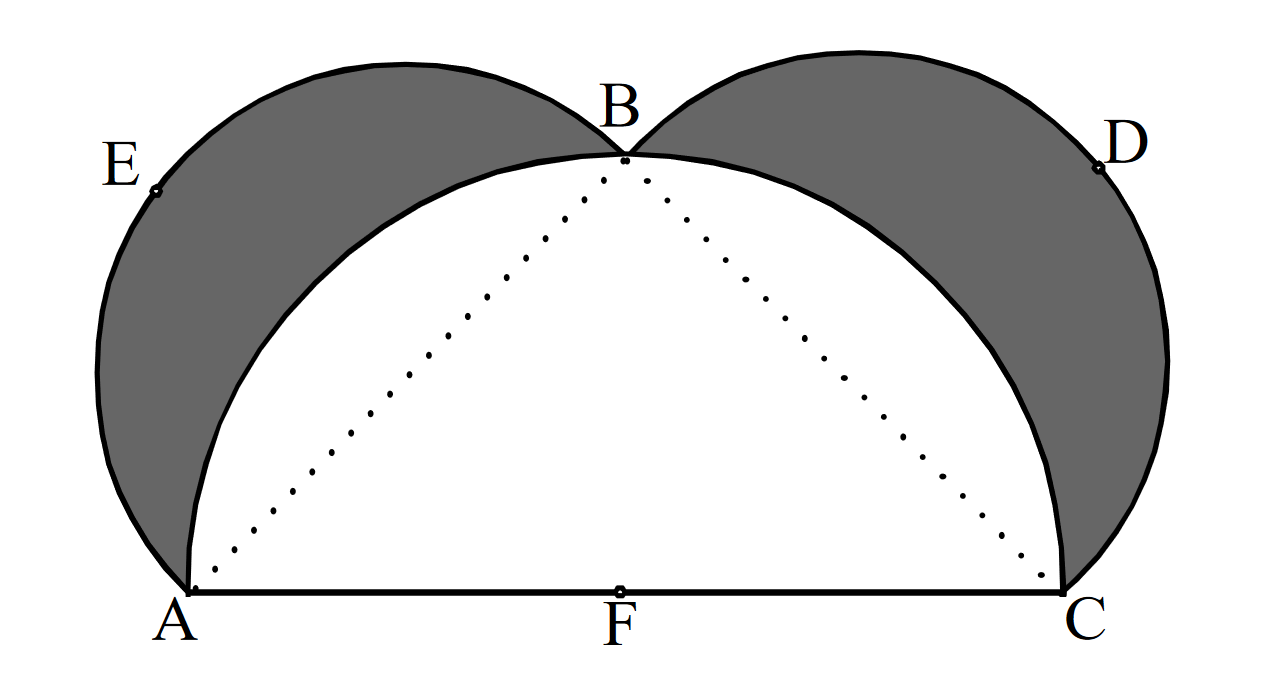
\includegraphics[width=3.5in]{mickeyMouse}
	\end{center}
	\end{problem}